\documentclass[oribibl]{llncs}
\usepackage{epsfig}
\usepackage{array}
\usepackage{multirow}
\usepackage{tikz}
\usepackage{color, colortbl}
\definecolor{Blue}{rgb}{0.69,0.88,0.99}
\definecolor{LightGreen}{rgb}{ 0.96,0.99, 0.9}
\usepackage{url}

\usepackage{amsmath,amssymb}
\usepackage{textcomp}
\usepackage{graphicx}
\usepackage{algorithm}
\usepackage{algpseudocode}
%\usepackage{wrapfigure}

\newcommand\numberthis{\addtocounter{equation}{1}\tag{\theequation}} % From: http://tex.stackexchange.com/questions/42726/align-but-show-one-equation-number-at-the-end
\newcommand{\norm}[1]{\left\lVert#1\right\rVert}
\newcommand{\argmin}{\operatornamewithlimits{argmin}}

%
\begin{document}

\title{Digit Detection Using Adaptive Spline Models}
\author{ Ansuya Ahluwalia\inst{1} \and Eric Kim\inst{1} \and Nicholas Brett Marcott\inst{1} }
\institute{University of California, Los Angeles \\* \email{ansuya@cs.ucla.edu, ekim@cs.ucla.edu, bmarcott@ucla.edu}}
\maketitle

\begin{abstract}

Automated handwriting detection remains an interesting yet challenging problem in the Vision field. Due to the curve-like nature of handwriting, it seems natural to consider approaches that directly model these curves. This project will investigate a particular approach from Hinton et. al \cite{Hinton92adaptiveelastic} that uses an elastic model to recognize digits. Each digit class is represented by a cubic spline. To classify a test image, an iterative algorithm performs an elastic match between the test image and each digit model - the digit class with the best score wins. Validation is performed against the handwritten digit dataset, MNIST \cite{mnist}.

\end{abstract}

\keywords{Digit Recognition, Cubic Spline, Elastic Match, Deformable Template}

\section{Introduction}

Automated handwriting detection is an interesting yet challenging problem in the Vision field. Traditional approaches to detection problems, such as template-based matching, are ineffective in this domain due to writing style variability: different people will write the same character in drastically different ways. Due to the curve-like nature of handwriting, however, it seems natural to consider approaches that attempt to model these curves.  
\\
\\
On the one hand, pure template matching is simple but brittle. To remain robust to variation, one must acquiare a large number of instances of each digit, resulting in many required image comparisons at test time.
On the other hand, using deformable templates increases the complexity of matching, but the number of matches decreases. In this project, we use deformable models based on cubic splines, containing a few parameters which captures many of the variations of a given digit. 
\\
\\
We investigate a particular approach from Hinton et. al \cite{Hinton92adaptiveelastic} that uses an elastic model to recognize digits. Each digit class is represented by a cubic b-spline with a particular ``home'' configuration. To classify a test image, an iterative algorithm  performs an elastic match between the test image and each digit class - the digit class with the best score wins. See Figure \ref{fig:bestFitEg} for an illustration of the classification approach. To remain invariant against factors such as translation, rotation, and scaling, all matching is performed in a canonical ``object frame''. Validation is performed against the publically-available handwritten digit dataset, MNIST \cite{mnist}.

\begin{figure}
\centering
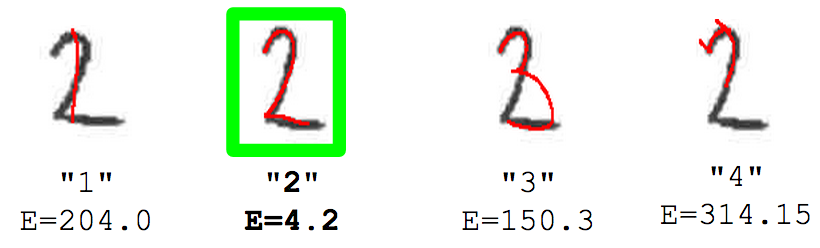
\includegraphics[height=3.25cm , width=12cm ]{bestFitEg}
\caption[]{Figure shows best fit model is the model with the lowest total energy (sum of deformation energy and fitting energy). Each digit model is matched to the test image, with energy scores to determine best fit.} 
\label{fig:bestFitEg}
\end{figure}

\section{Related Work}
 
Prominent amount of work in the field of handwriting recognition revolves around neural networks (recurrent, hierarchical, deep forward etc.). Neural networks learn from an image training set for character recognition. Each neural network uniquely learns features that differentiate training images. The target image is classified based on the similarity in properties with the training images. Neural networks are quick to set up but can be inaccurate if unimportant properties are learnt in context to the target data. 
\\
\\
For discrete character recognition, neural networks are trained on weights of template neural nets that generate the character (digit/ alphabet) with highest likelihood. Normalization is used to label the data. However, this system can only be applied to recognition of cursive and unconstrained words if templates of each word are made. This is due to the problem of character segmentation that exists in cursive and unconstrained handwriting. To handle unconstrained words, most researchers use Time-Delay Neural Networks (TDNN's) to generate labels for segments of data \cite{mantas1986overview}. In \cite{tddnn}, authors use a time-delay neural network to estimate a posteriori probabilities for characters in a word. A hidden markov model segments the word in a way that optimizes the global word score, using a dictionary in the process.
\\
\\
A lot of research has been in developing advanced algorithms for handwriting recognition using neural networks and hidden markov models. In \cite{LeCun:1989:BAH:1351079.1351090}, authors use backpropagation to recognize handwritten zip codes. Researchers have also developed novel, biologically motivated approaches to classify handwritten characters. Dystal ( Dynamically Stable Associative Learning) is one such neural network algorithm \cite{Blackwell1992655}. In \cite{97912}, researchers use neocognitron, a neural network model for deformation-invariant visual pattern recognition, for handwritten alphanumeric character recognition. \cite{541414} incorporate HMM's into a complex stochastic language model for handwriting recognition. The pattern elements of the handwriting model are subcharacter stroke types modeled by HMMs. These HMMs are concatenated to form letter models, which are further embedded in a stochastic language model. \cite{Bengio95lerec:a} use a neural network/ HMM hybrid model for on-line handwriting recognition. They also employ EM algorithm in their approach. They perform a word-level normalization by fitting a model of the word structure using the EM algorithm. 
\\
\\
Deformable models are efficient for characterizing handwritten digits since they have
relatively few parameters and are able to capture many variations in digit instances. We investigate the system described in \cite{Hinton92adaptiveelastic} that uses learned digit models consisting of splines whose shape is governed by a small number of control points. This method uses a single model for each digit class. As as extension to their work in \cite{Hinton92adaptiveelastic}, authors developed multi-models for each digit class, with little computational overhead, to better characterize the variations in the instances of each digit \cite{revow1993using}. 


\section{Methodology}
\label{sec:methodology}

In this section we discuss the details for performing digit recognition.
As these digits are created by a series of strokes, or curves, a cubic B-spline curve is a natural representation to model the curves' "ideal" shape. As a summary of the fitting process, a model representing each digit is fit to an input image. The image is then classified as the digit represented by the model that fits best to the image without excessive deformation.

\subsection{Digit model}
In this project, cubic B-spline models are defined for only two digit classes, twos and threes. Both of these models are defined using eight control points, hence each segment of the curve is affected by only four of the control points. Along the curve, there are evenly spaced "ink generators" or "beads," which are modeled by bi-variate Gaussian distributions. These beads are used to calculate the probability of an inked pixel being generated by a particular bead. In this way inked pixels are much more likely to be generated by a neighboring bead, but are still affected by the other beads. 
\\
\\
\\
Similar to other inverse problems, the objective function is a balance between some regularization term and a data fit term. In this project, the regularization term is a penalty for how much the b-spline deviates from its original model position. The data fit term is calculated based on each inked pixels probability of being generated by the gaussians along the spine of the curve. The equations are as below:

\begin{equation*}
\numberthis \label{eq:E_total}
    E_{tot} = E_{def} + E_{fit}
\end{equation*}

$$ E_{def} =  \sum_{CP}{(\textbf{x}_{home} - \textbf{x}_{new})^2}$$ 
This is the sum of the squared differences of the control point positions before and after deformation.

$$ E_{fit} = -\frac{N_0}{N_B}\sum_{i \in inked}^{N_B}{log(f(y_i))}  $$
\\
Where $N_0$ is a "standard" number of pixels and $N_B$ is the number of inked pixels.

$$ f(y) =  \frac{\pi_n}{A} + \frac{1-\pi_n}{B}\sum_{G}{f_g(y)}$$ 
\\
Where $f_g(y)$ is the value of a pixel located at position y under a bi-variate Gaussian distribution g, and $\pi_n$ is the relative weight a pixel has by being generated randomly from uniform noise versus by the ink generators. In this way, the equation for $f(y)$ is a mixture model that accounts for a pixel being generated either by uniform noise or by an ink generator.\\


\subsection{EM algorithm}
To minimize the objective function, the total energy, an EM algorithm is used. In the E step of the algorithm, the "responsibilities" of each of the beads is calculated and held fixed for the M step. These responsibilities are the probability of a pixel being generated by a single ink generator normalized by the total probability of being generated. 

$$ r_g(y) = \frac{f_g(y)}{f(y)} $$
\\
The maximization contains two steps. The first step maximizes the total energy with fixed responsibilities, finding the balance between the deformation and data fit terms. The second step updates an affine transformation that absorbs some of the unneeded deformation penalties due to natural deviations such as scaling and rotation. The difference in the control point positions used for calculating the $E_{def}$ term are computed in the object based frame. The transformation from the image based frame to the object based frame is calculated as mentioned in the second M step.
\\
\\
A fixed annealing schedule is used for the EM algorithm. At each stage of the annealing schedule, the variance of each of the ink generators is decreased and the number of them is increased to account for finer detail in the image. This process may stop either when the total energy has not changed by a set threshold or when all the iterations are complete. The process may converge to local maximum based on initial conditions.

\subsection{Digit Classification}
\label{sec:classify}

In this project, we investigated two methods of performing digit classification.
Given an input image, we perform the elastic matching algorithm from Section \ref{sec:methodology}. 
In addition to the spline parameters of the fit, the algorithm also outputs the energy, or score, of the fit, according to Equation \ref{eq:E_total}, reproduced below:

\begin{equation*}
    E_{tot} = E_{def} + E_{fit}
\end{equation*}    

As $E_{tot}$ is a measure of how well a digit model fits to the input image, one natural classification method is to simply output the label of the best-fitting model.
In other words, the classificaton is performed as:
\begin{equation*}
\numberthis \label{eq:class1}
\text{label} = \argmin_{m \in Models}{E_{tot}^{(m)}}
\end{equation*}

Upon examining several digit fits, we discovered that the $E_{def}$ and $E_{fit}$ terms seemed to be on different scales.
With this in mind, we considered performing classification on the weighted sum:
\begin{equation*}
\numberthis \label{eq:class2}
\text{label} = \argmin_{m \in Models}{E_{def}^{(m)} + \alpha \cdot E_{fit}^{(m)}}
\end{equation*}
Where $\alpha$ is a tunable parameter that controls the relative importance between $E_{def}$ and $E_{fit}$.
Note that the first classification rule (Equation \ref{eq:class1}) is a special case of (Equation \ref{eq:class2}), with $\alpha = 1.0$.

\section{Results}

We evaluated the digit classifier on a subset of the MNIST Handwritten Digit Database \cite{mnist}.
The dataset consists of labeled graylevel, pre-segmented, centered, 20x20 images.
See Figure \ref{fig:mnist_imgs} for several example images.

\subsection{Preprocessing}
\label{sec:preproc}

Following the authors of \cite{Hinton92adaptiveelastic}, we first apply several basic preprocessing steps to the input digit images to obtain binary, thinned images.
First, the images are thresholded using Otsu's method, yielding a binary image with (hopefully) spurious details removed.
See Figure \ref{fig:mnist_imgs} to see the results of the preprocessing operations.

\subsection{Evaluation}

First, we determined the optimal setting for the $\alpha$ parameter (see Section \ref{sec:classify}) by doing a grid-search on a separate validation set of 50 images.
For the other parameters ($N_0$, $\pi_N$), we elected to use the values that the authors suggest in \cite{Hinton92adaptiveelastic}, as we found that they worked well in practice.

We evaluated the digit classification algorithm on 150 images from MNIST.
Results are found in Table \ref{tab:results}.
In our simple MATLAB implementation, it takes roughly 110 seconds to classify an image.
Much of the time is spent solving a least-squares problem with a general-purpose solver\footnote{CVX: http://cvxr.com/cvx/}.


\begin{figure*}
\centering
\begin{tabular}{cc}
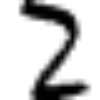
\includegraphics[width=.2\linewidth]{figs/Imnist_3749.png} & 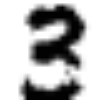
\includegraphics[width=.2\linewidth]{figs/Imnist_1960.png} \\
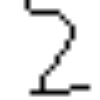
\includegraphics[width=.2\linewidth]{figs/Imnist_proc_1.png} & 
\includegraphics[width=.2\linewidth]{figs/Imnist_proc_16.png} \\
\end{tabular}
\caption{Top: Example images from MNIST. Bottom: Result of applying preprocessing operations (Section \ref{sec:preproc}).}
\label{fig:mnist_imgs}
\end{figure*}

\begin{table}
\centering
  \begin{tabular}{ l || c | c | c }
  & Accuracy & Correct & Incorrect \\ \hline
    Original &  FOO\% & FOO & FOO \\ \hline
    Weighted Sum ($\alpha = FOO$) & FOO\% & FOO & FOO \\
  \end{tabular}
\vspace{1em}
\caption{Classification results on MNIST. ``Original'' corresponds to the first classifier defined by Equation \ref{eq:class1}. ``Weighted Sum'' corresponds to the classifier defined by Equation \ref{eq:class2}.}
\label{tab:results}
\end{table}



\subsection{Discussion}

Model-based top-down approaches such as the one presented here leads to easily interpretable results.
After fitting, the deformable digit spline models provide a powerful interpretation of the input image.
However, this power comes at a cost - the iterative algorithm is a very expensive online process.
Further, the recognition rates listed in this report are fairly lack-luster, considering that performance on the MNIST dataset has effectively saturated at near-perfect accuracy.
For instance, Ciresan et. al. reports an error rate as low as 0.23\% on MNIST by utilizing a deep neural network \cite{ciresan}.

Yet, it is worth noting the attractive qualities of model-based methods such as the one explored here.  
The iterative fitting process seeks to best explain the input image with respect to a set of known digit spline models.
As a result, the algorithm richly describes the image in a principled manner.
On the other hand, approaches such as \cite{ciresan} train classifiers with the explicit goal of classification.
Often, such approaches treat the problem purely as a pattern recognition problem, and don't care to ``explain'' the images.
Thus, in a philosophical sense it is difficult to compare the two approaches, as the goals are inherently different.

\section{Conclusion}

We have investigated a model-based approach to digit recognition that iteratively fits deformable spline models to input digit images, yielding easily interpretable results.


 \bibliography{project-bibfile}
\bibliographystyle{plain}

\end{document}
